\documentclass[a4paper,12pt]{article}
\addtolength{\oddsidemargin}{-1.cm}
\addtolength{\textwidth}{2cm}
\addtolength{\topmargin}{-2cm}
\addtolength{\textheight}{3.5cm}
\newcommand{\HRule}{\rule{\linewidth}{0.5mm}}
\makeindex

\usepackage{longtable}
\usepackage[pdftex]{graphicx}
\usepackage{makeidx}
\usepackage{hyperref}
\usepackage{float}
\usepackage{verbatim}
\usepackage[space]{grffile}
\usepackage[export]{adjustbox}

\hypersetup{
    colorlinks=true,
    linkcolor=blue,
    filecolor=magenta,      
    urlcolor=cyan,
}


% define the title
\author{IMAPKD}
\title{ User Manual}
\begin{document}
\setlength{\parskip}{6pt}

% generates the title
\begin{titlepage}

\begin{center}
% Upper part of the page       
\includegraphics[width=1\textwidth]{./University_of_Pretoria_Logo.PNG}\\[0.4cm]  
\textsc{\LARGE COS 301}\\[0.9cm]
\textsc{\LARGE Department Of Computer Science}\\[0.3cm]

%Title

\HRule \\[0.4cm]
{ \huge \bfseries User Manual}\\[0.1cm]
\HRule \\[0.4cm]  

% Group Members 

\begin{minipage}{0.4\textwidth}
\begin{flushleft} \large

\emph{\Large Group Members:}\\[0.4cm]    
\emph{}\\
{\Large Diana {Obo}} \\
\emph{}\\
\emph{}\\
{\Large Priscilla {Madigoe}}\\
\emph{}\\
\emph{}\\
{\Large Kudzai {Muranga}} \\
\emph{}\\
\emph{}\\
{\Large Sandile {Khumalo}}\\
\emph{}\\
\emph{}\\

\end{flushleft}
\end{minipage}
\begin{minipage}{0.4\textwidth}
\begin{flushright} \large

\emph{ \Large Student numbers:} \\[0.4cm]  
\emph{}\\
{\Large u13134885}\\
\emph{}\\
\emph{}\\
{\Large u13049128}\\
\emph{}\\
\emph{}\\
{\Large u13278012}\\
\emph{}\\
\emph{}\\
{\Large u12031748}\\
\emph{}\\
\emph{}\\

\end{flushright}
\end{minipage}

% bottom section of title page

{\large \today}
\end{center}
\end{titlepage}
\renewcommand{\thesection}{\arabic{section}}

\newpage
\begin{center}
\textsc{\Large IMPAKD link}\\[0.5cm]
For further references see \href{https://github.com/u13278012/IMPAKD/}{gitHub}.
\today
\end{center}
\cleardoublepage
\thispagestyle{empty}
\tableofcontents
%\newpage
%\tableofcontents{}

\newpage
\setcounter{page}{3} 
\section{Introduction}


\section{Vision}


\section{System Overview}


\section{Installation}


\section{Getting Started}

\newpage

\section{Using The System}

%Main Page - Navigation Pane
 
\subsection{Main Page - Navigation Pane}
	\begin{figure}[H]
		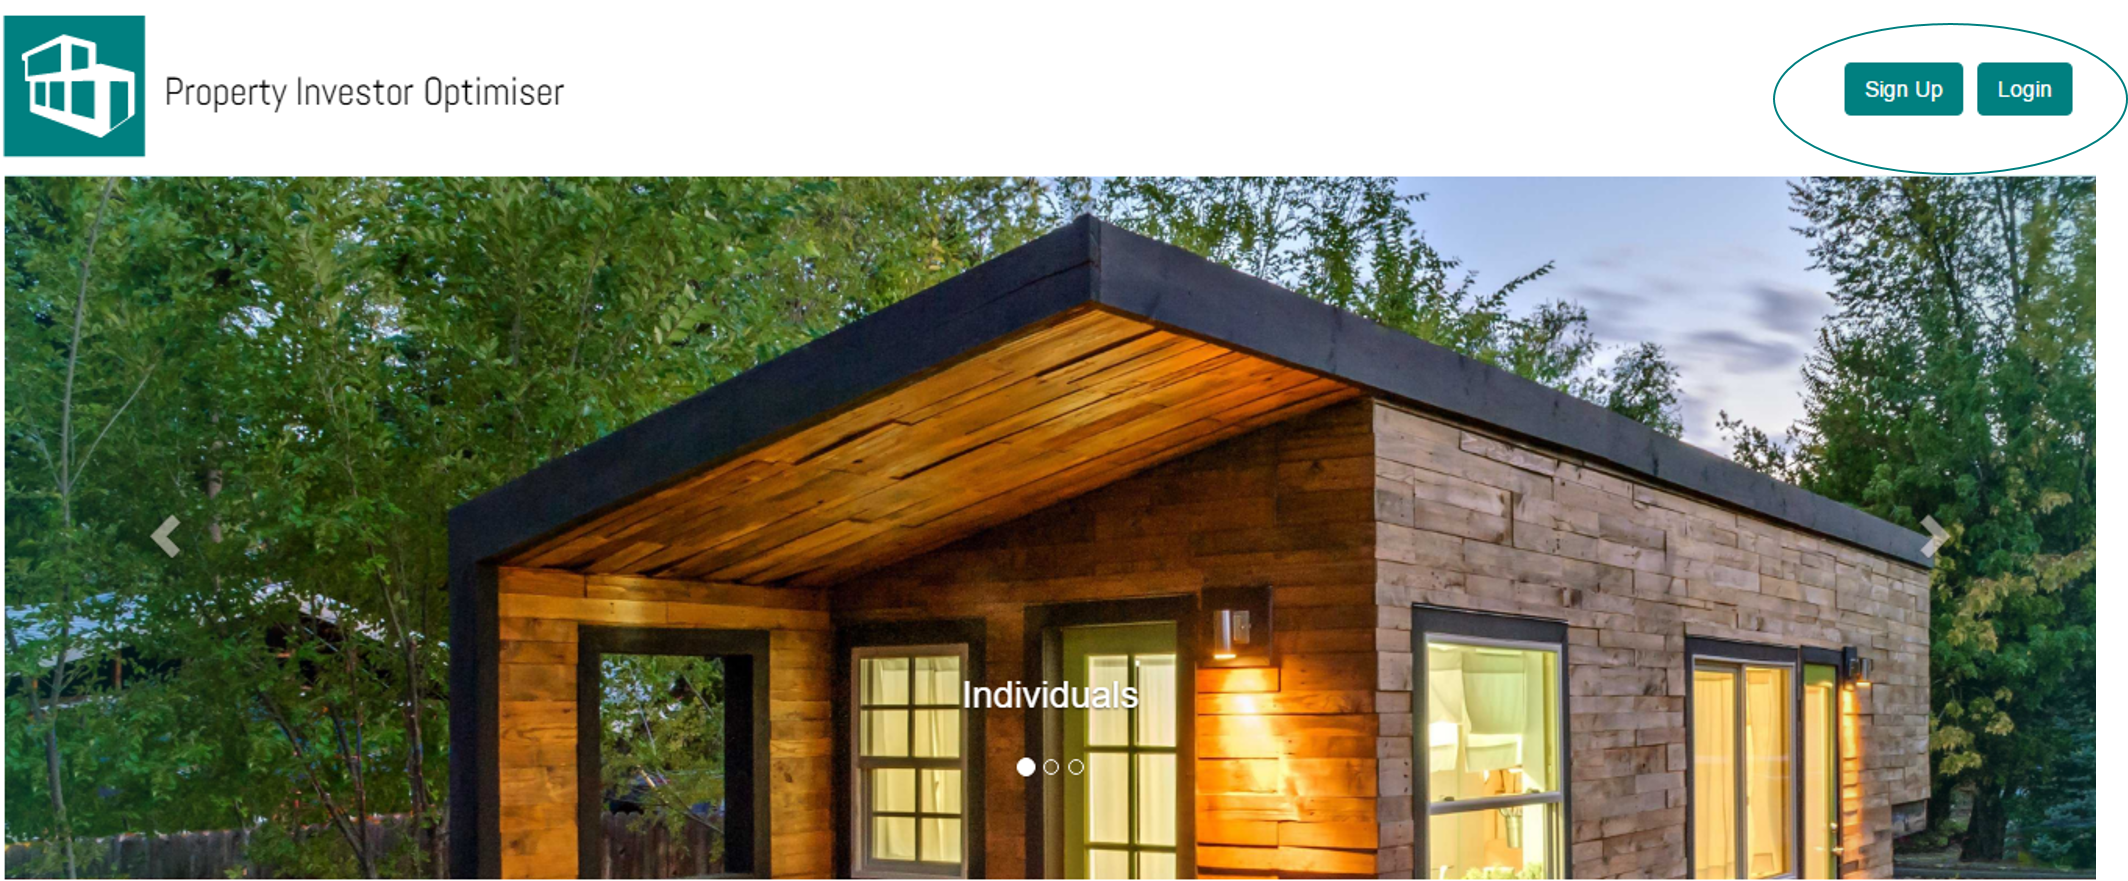
\includegraphics[width=0.9\linewidth, center]{./System/Navigation.PNG}\\[0.4cm]  
		\caption{Main Page - Navigation Pane}
	\end{figure}
This page will be the first page the user will come across when visiting the website. It contains two buttons: One to "login" and another to "sign-up" so that the user can access and use the system. It also contains information about the purpose and the functionality of the website.

%Register Page
\subsection{Register Page}
	\begin{figure}[H]
		\includegraphics[width=0.9\linewidth, center]{./System/Register.PNG}\\[0.4cm]  
		\caption{Register Page}
	\end{figure}
This page is shown when the user selects the "register" button on the aforementioned "main page". It is meant for people who do not have an account on the website and would like to use the system. This will enable the user to create a profile and will then be able to use the system . The user will use this page to gain access into the system and will be redirected to the "home page" once they have successfully registered.

%Login Page
\subsection{Login Page}
	\begin{figure}[H]
		\includegraphics[width=0.9\linewidth, center]{./System/Login.PNG}\\[0.4cm]  
		\caption{Login Page}
	\end{figure}
This page is shown when the user selects the "login" button on the aforementioned "main page". It is meant for people who have already created an account and have a valid profile on the website. The user will use this page to gain access into the system and will be redirected to the "home page" once they have successfully logged in.

\end{document}

